% coding:utf-8

%----------------------------------------
%FOSAMATH, a LaTeX-Code for a mathematical summary for basic analysis
%Copyright (C) 2013, Daniel Winz, Ervin Mazlagic, Adrian Imboden, Philipp Langer

%This program is free software; you can redistribute it and/or
%modify it under the terms of the GNU General Public License
%as published by the Free Software Foundation; either version 2
%of the License, or (at your option) any later version.

%This program is distributed in the hope that it will be useful,
%but WITHOUT ANY WARRANTY; without even the implied warranty of
%MERCHANTABILITY or FITNESS FOR A PARTICULAR PURPOSE.  See the
%GNU General Public License for more details.
%----------------------------------------

% coding:utf-8
\section{Maschenstromverfahren}

\begin{itemize}
	\item Alle realen Quellen in Spannungsquellen wandeln
	\item Maschen legen und nummerieren ($M_1$, $M_2$, $M_3$ ...$M_n$)
	\item Baum bilden (Baum bedeutet hier ein Strang, welcher alle Knoten berührt und durchgehend verbunden ist. Dieser muss keine \textit{Schlange} darstellen, sondern darf auch sternförmig etc. sein.
	\item Matrix aufstellen
	\item Links alle Maschen auflisten
	\item Oben alle Ströme der Quellen eintragen welche zwischen Knoten liegen (nicht jener die innerhalb des Baumes liegen)
	\item Hauptdiagonale ausfüllen:\\ Hierzu sind alle Widerstandswerte zu summieren welche in entsprechender Masche liegen.
	\item Restliche Matrix ausfüllen:\\ Hierzu sind alle Widerstandswerte einzutragen welche zu zwei Maschen gehören einzutragen. Das Vorzeichen ist positiv zu wählen, falls die Maschenpfeilrichtung die selbe ist, sonst negativ.
	\item In der rechten Spalte Spannungsquellen eintragen. Das Vorzeichen ist dabei positiv, falls die Maschenpfeilrichtung entgegen der Spannungspfeilrichtung ist, sonst negativ.
\end{itemize}

\newpage

\subsection{Beispiel}
\begin{figure}[h!]
\centering
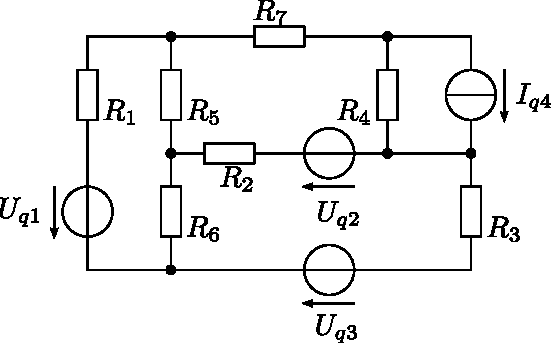
\includegraphics[width=0.55\textwidth]{mastro_sch.pdf}

\vspace{5mm}

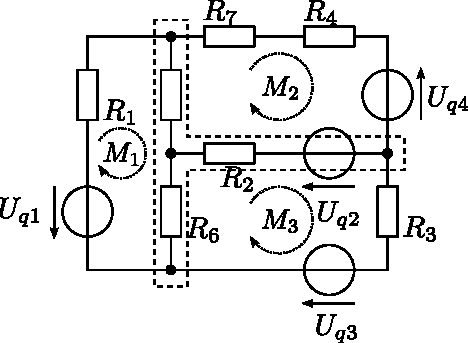
\includegraphics[width=0.50\textwidth]{mastro_sch_2.pdf}
\label{sch:mastro}
\caption{Schaltung zum Maschenstromverfahren}
\end{figure}

\begin{figure}[h!]
\footnotesize
\[ \begin{array}{c|ccc||c}

M	& I_1 & I_4 & I_3 & U \\
\hline &&&& \\
M_1 	& R_1 + R_2 + R_3 	& -R_5 				& -R_6 			& U_{q1} \\
&&&& \\
M_2 	& -R_5 			& R_2 + R_4 + R_5 + R_7 	& -R_2 			& U_{q4} \\
&&&& \\
M_3 	& -R_6 			& -R_2 				& R_2 + R_3 + R_6 	& -U_{q3} \\
\end{array}
\]
\normalsize
\caption{Matrix zu Abb.~\ref{sch:mastro}}
\end{figure}
